% This file was created with tikzplotlib v0.10.1.
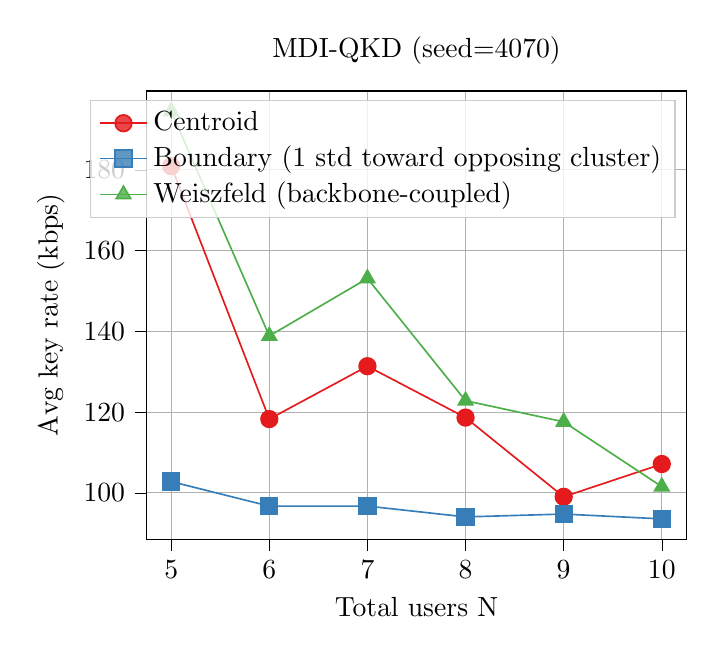
\begin{tikzpicture}

\definecolor{crimson2282628}{RGB}{228,26,28}
\definecolor{darkgray176}{RGB}{176,176,176}
\definecolor{lightgray204}{RGB}{204,204,204}
\definecolor{mediumseagreen7717574}{RGB}{77,175,74}
\definecolor{steelblue55126184}{RGB}{55,126,184}

\begin{axis}[
legend cell align={left},
legend style={fill opacity=0.8, draw opacity=1, text opacity=1, draw=lightgray204},
tick align=outside,
tick pos=left,
title={MDI-QKD (seed=4070)},
x grid style={darkgray176},
xlabel={Total users N},
xmajorgrids,
xmin=4.75, xmax=10.25,
xtick style={color=black},
xtick={4,5,6,7,8,9,10,11},
xticklabels={
  \(\displaystyle {4}\),
  \(\displaystyle {5}\),
  \(\displaystyle {6}\),
  \(\displaystyle {7}\),
  \(\displaystyle {8}\),
  \(\displaystyle {9}\),
  \(\displaystyle {10}\),
  \(\displaystyle {11}\)
},
y grid style={darkgray176},
ylabel={Avg key rate (kbps)},
ymajorgrids,
ymin=88.5145955098621, ymax=199.554724874201,
ytick style={color=black},
ytick={80,100,120,140,160,180,200},
yticklabels={
  \(\displaystyle {80}\),
  \(\displaystyle {100}\),
  \(\displaystyle {120}\),
  \(\displaystyle {140}\),
  \(\displaystyle {160}\),
  \(\displaystyle {180}\),
  \(\displaystyle {200}\)
}
]
\addplot [semithick, crimson2282628, mark=*, mark size=3, mark options={solid}]
table {%
5 180.946146680982
6 118.28633789807
7 131.380645377894
8 118.657304346459
9 99.0368313411155
10 107.14822748488
};
\addlegendentry{Centroid}
\addplot [semithick, steelblue55126184, mark=square*, mark size=3, mark options={solid}]
table {%
5 102.806765558629
6 96.7131824139206
7 96.7298594605134
8 94.0548725364098
9 94.7579283033431
10 93.5618741173321
};
\addlegendentry{Boundary (1 std toward opposing cluster)}
\addplot [semithick, mediumseagreen7717574, mark=triangle*, mark size=3, mark options={solid}]
table {%
5 194.507446266731
6 138.868189720038
7 153.113164051521
8 122.830733185938
9 117.602420796404
10 101.549692797282
};
\addlegendentry{Weiszfeld (backbone-coupled)}
\end{axis}

\end{tikzpicture}
